\subsection{Mail Script}
\begin{figure}
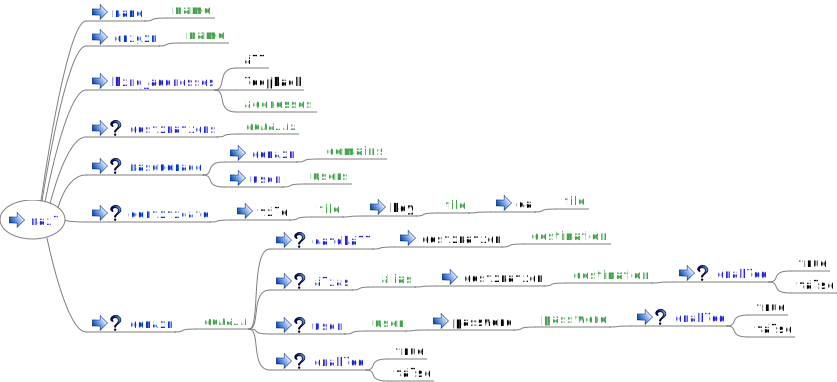
\includegraphics[width=0.9\textwidth]{mail_service_script}
\label{fig:mail_script_statements}
\caption{Mail Script Statements}
\end{figure}


\TheStatement{mail}
\TheStatement*[mail]{mail \{ name origin masquerade certificate domain \}}

Entry point in the mail script.

\TheStatement[mail:name]{name}
\TheStatement*[mail!name]{name \Arg{name}}

The domain \Arg{name} of the server.

\TheStatement[mail:origin]{origin}
\TheStatement*[mail!origin]{origin \Arg{name}}

The domain \Arg{name} that locally-posted mail appears to come
from, and that locally posted mail is delivered to.

\TheStatement[mail:bind_addresses]{bind\_addresses}
\TheStatement*[mail!bind\_addresses]{bind\_addresses all|loopback|\Arg{addresses}}

The network interface addresses that this mail system receives mail on.
Specify all to receive mail on all network interfaces,
and loopback to receive mail on loopback network interfaces only. Otherwise
a list of \Arg{addresses} can be specified.
Defaults to all.

\TheStatement[mail:destinations]{destinations}
\TheStatement*[mail!destinations]{destinations \Arg{domains}}

Additional list of \Arg{domains} that are delivered to local mail users.
Do not specify names of virtual domains, those domains are specified
in the \Statement*[mail:domain]{domain} statements.

\TheStatement[mail:masquerade]{masquerade}
\TheStatement*[mail!masquerade]{masquerade \{ domains user \}}

Starts a list of domains and users to masquerade. Masqueraded domains and
users are stripped off of their subdomain structure in email addresses.
A domain name prefixed with ``!'' means do not masquerade this domain
or its subdomains.

\TheStatement[mail:masquerade:domains]{domains}
\TheStatement*[mail!masquerade!domains]{domains \Arg{domains}}

Sets the \Arg{domains} to masquerade.

\TheStatement[mail:masquerade:user]{user}
\TheStatement*[mail!masquerade!user]{user \Arg{users}}

Sets the list of \Arg{users} that are not subjected to address masquerading.

\TheStatement[mail:certificate]{certificate}
\TheStatement*{certificate file key ca}

Defines the location of the certificate files for TLS.

\TheStatement[mail:certificate:file]{file}
\TheStatement*[mail!certificate!file]{file \Arg{file}}

The location of the certificate file.

\TheStatement[mail:certificate:key]{key}
\TheStatement*[mail!certificate!key]{key \Arg{file}}

The location of the certificate key file.

\TheStatement[mail:certificate:ca]{ca}
\TheStatement*[mail!certificate!ca]{ca \Arg{file}}

The location of the certificate CA file.

\TheStatement[mail:domain]{domain}
\TheStatement*[mail!domain]{domain \Arg{domain} catchall alias user enabled \}}

Adds domains that are known to the mail server. A domain can have a catch-all
alias, other aliases, users and an enabled flag. The current domain is appended
to aliases and users without a domain part. So for example the user ``xandros''
in the ``blobber.org'' domain will have the address ``xandros@blobber.org''.

\TheStatement[mail:domain:catchall]{catchall}
\TheStatement*[mail!domain!catchall]{catchall destination: \Arg{destination}}

Creates a catch-all alias to the current destination. The catch-all is equal
to the alias ``@domain'', where the ``domain'' is the current domain name.

Example:

\begin{compactitem}
\item ``\code{catchall destination: "@blobber.org"}''
\item ``\code{catchall destination: "xandros@blobber.org"}''
\end{compactitem}

\TheStatement[mail:domain:alias]{alias}
\TheStatement*[mail!domain!alias]{alias \Arg{alias}, destination: \Arg{destination}}

Creates a new alias with the specified destination. The current domain is appended
to the aliases without a domain part. So for example the alias ``karl''
in the ``blobber.org'' domain will have the address ``karl@blobber.org''.

Example:

\begin{compactitem}
\item ``\code{alias "karl", destination: "karl.vovianda@galias.com"}''
\item ``\code{alias "postmaster@blobber.org", destination: "postmaster@\\localhost"}''
\end{compactitem}

\TheStatement[mail:domain:enabled]{enabled}
\TheStatement*[mail!domain!enabled]{enabled true|false}

Sets the enabled flag on a domain, user or alias. Disabled domains, users or
aliases are ignored by the mail server.

\TheStatement[mail:domain:user]{user}
\TheStatement*[mail!domain!user]{user \Arg{user}, password: \Arg{password}}

Adds a new user with the specified password for the domain.
Only virtual users are created or their passwords changed.
Local account management is not in scope with the mail service.
The current domain is appended to the users without a domain part. 
So for example the user ``karl'' in the ``blobber.org'' domain will 
have the address ``karl@blobber.org''.

